% !TeX spellcheck = en_US
\documentclass[letterpaper,12pt,twoside]{report}
\usepackage{fancyhdr}
\usepackage{fullpage}
\usepackage{tikz}
\usepackage{amsmath}

\begin{document}
	\pagestyle{fancy}
	\fancyhf{}
	\fancyhead[L]{Day 15}
	\fancyhead[R]{\textit{The Calendar Project}}
	\fancyfoot[L]{Citations Involved: ???}
	
	% Problem
	\paragraph{Problem}
	\begin{quote}
		\textsf{A line $p$ with positive slope
			intersects the parabola $y=x^2$
			at $A(x_1, y_1)$ and $B(x_2, y_2)$, where $y_2 = y_1 + 16$. If $A$ and $B$ are $8\sqrt{5}$ units apart, what is the equation of the line $p$ in y-intercept form?}
	\end{quote}
	
	% Graphics
	\begin{center}
		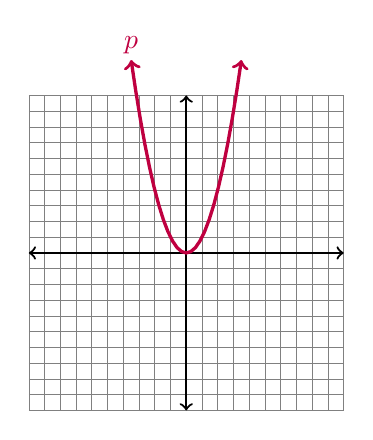
\begin{tikzpicture}[scale=0.2]
		
		\draw[help lines] (-10,-10) grid (10,10);
		\draw[<->][thick] (0,10) -- (0,-10);
		\draw[<->][thick] (-10,0) -- (10,0);
		
		\draw[purple, very thick, <->, domain=-3.5:3.5] plot (\x, {\x*\x});
		\node[purple, above] at (-3.5, 12) {$p$};
		\end{tikzpicture}
	\end{center}
	
	% Reasoning
	\paragraph{Reasoning}
	\begin{quotation}
		
		???
		
	\end{quotation}
	
	\paragraph{External References}
	
	\begin{enumerate}
		\item ???
	\end{enumerate}
	
\end{document}